\chapter{Collaborative Tasks}
\label{chapter:colab-tasks}

\section{Hand Guiding}

\par So far, it has been explained how to obtain a compensated \ac{ft} measurement in order to obtain \acf{hgft}, which is caused by the user. This value is used to move the robot in the direction that it is applied. For this to happen, this values felt on the \ac{ft} reference frame need to be converted to a velocity vector, referenced on the base frame of the robot. 

\subsection{\ac{hgft} to \ac{eef} Velocity}

\par \ac{hgft} should only converted in robot motion when it reaches a certain threshold, otherwise, it should be zero. It should also exist a way to define the ration of conversion between \ac{ft} and velocity To achieve this behavior, the \ac{hgft} is controlled according to \autoref{eq:f_thresh} and \autoref{eq:t_thresh}.

\begin{multicols}{2}
    \begin{equation}
        \mathbf{f_i} =
        \begin{cases}
          \frac{f_i - f_{th}}{f_{div}} & f_i > f_{th}\\
          \frac{f_i + f_{th}}{f_{div}} & f_i < f_{th}\\
          0 & \text{otherwise}
        \end{cases}
        \label{eq:f_thresh}
    \end{equation}\break
    \begin{equation}
        \mathbf{t_i} =
        \begin{cases}
          \frac{t_i - t_{th}}{t_{div}} & t_i > t_{th}\\
          \frac{t_i + t_{th}}{t_{div}} & t_i < t_{th}\\
          0 & \text{otherwise}
        \end{cases}
        \label{eq:t_thresh} 
    \end{equation}
\end{multicols}

\noindent Where $\mathbf{f_i}$ and $\mathbf{t_i}$ are \ac{ft} components, $\mathbf{t_{th}}$ and $\mathbf{f_{th}}$ are \ac{ft} threshold parameters, and $\mathbf{t_{div}}$ and $\mathbf{f_{div}}$ are ratio constants that define the conversion between \ac{ft} and velocity.

\subsubsection{Force to Linear Velocity}

\par It is done by creating a pose with the force measurement as the position component, and transforming this pose with the rotation matrix of the \ac{ft} sensor frame. The resulting pose position can be directly used as global velocity. \autoref{eq:force_to_linear_vel} is used to calculate the linear velocity from the \ac{hg} force.

\begin{equation}
    \vec{\mathbf{V_{lin}}} = R^b_e \cdot R^e_s \cdot P_{force}
    \label{eq:force_to_linear_vel}
\end{equation}

\noindent Where $\mathbf{R^b_e}$ is the rotation matrix of the \ac{eef} frame in relation to the robot base frame, $\mathbf{R^e_s}$ is a constant rotation matrix of the sensor frame in relation to the \ac{eef} frame, and $P_{force}$ is a point with the force measurements as its coordinates. $\vec{\mathbf{V_{lin}}}$ is obtained as a cartesian points which can directly be used as a linear velocity vector in the robot base frame.

\subsubsection{Torque to Angular Velocity}

\par It is done by creating a pose with the torque measurement as the orientation component, transforming this orientation with the rotation matrix of the \ac{ft} sensor frame, and with this orientation, rotate the inverse rotation of the \ac{ft} sensor frame. \autoref{eq:force_to_linear_vel} is used to calculate the angular velocity from the \ac{hg} torque.

\begin{equation}
    \vec{\mathbf{V_{ang}}} = (R^b_e \cdot R^e_s \cdot R_{torque}) \cdot (R^b_e \cdot R^e_s)^{-1}
    \label{eq:torque_to_angular_vel}
\end{equation}

\noindent Where $\mathbf{R^b_e}$ is the rotation matrix of the \ac{eef} frame in relation to the robot base frame, $\mathbf{R^e_s}$ is a constant rotation matrix of the sensor frame in relation to the \ac{eef} frame, and $R_{torque}$ is a rotation with the torque measurements as its elements. $\vec{\mathbf{V_{ang}}}$ is obtained as a cartesian rotation which can directly be used as angular velocity in the robot base frame.

\subsection{\ac{eef} Velocity to Joint Speed}

\par Explain here the conversion from eef\_velocity to o joint speed. say that here is the first time that this conversion is talked about 

% ADD: Reference this subsection from other places mainly end of chapter 3 and 4


\begin{figure}[h]
    \centering
    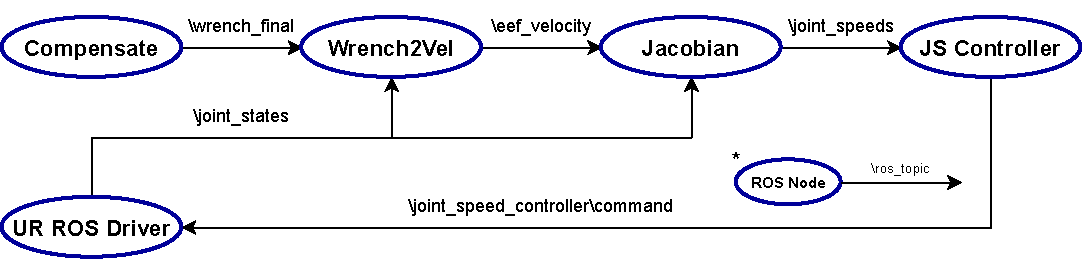
\includegraphics[width=\linewidth]{figs/chp4/ros_hg_arch.pdf}
    \caption{\ac{ros} architecture of the \ac{hg} task}
    \label{fig:ros_hg_arch}
\end{figure}

\section{Object Transfer}

\par Explain the execution of this task... explain the importance of a parametrized skill because the user can define the pick and deliver place and the task works every time
\par explain the intrinsic details of the deliver method

\section{Object Manipulation}

\par This task is more complex, since after gripping a lot of things happen, the controllers are switched, the robot is moved 5 cm upwards to make the user not interact with the gripper beacuse it will calibrate the weight, after the weight is calibrated the hand guide feature is back online with the new calibrated weight on the ft theory model... the robot will continue in hand guide until a double tap on y is perform, making the robot release the object and set the weight to zero... when the robot releases the weight it will also zero de ft sensor because as said previously, interactiong with the sensor can cause deveiations on the measurements

\section{Collision Free Execution of an Industrial Task}

\par definition of an industrial task, turn on collision avoidacne algorithm, now the joint speed controller will listen to the pf controller and the robot will be performing the task until an interaction is made with it

\section{Collaborative State Machine}

\par explain the intrinsic detail of the state machine
\par good for overall system architecture and description of the state machine

\begin{figure}[h]
    \centering
    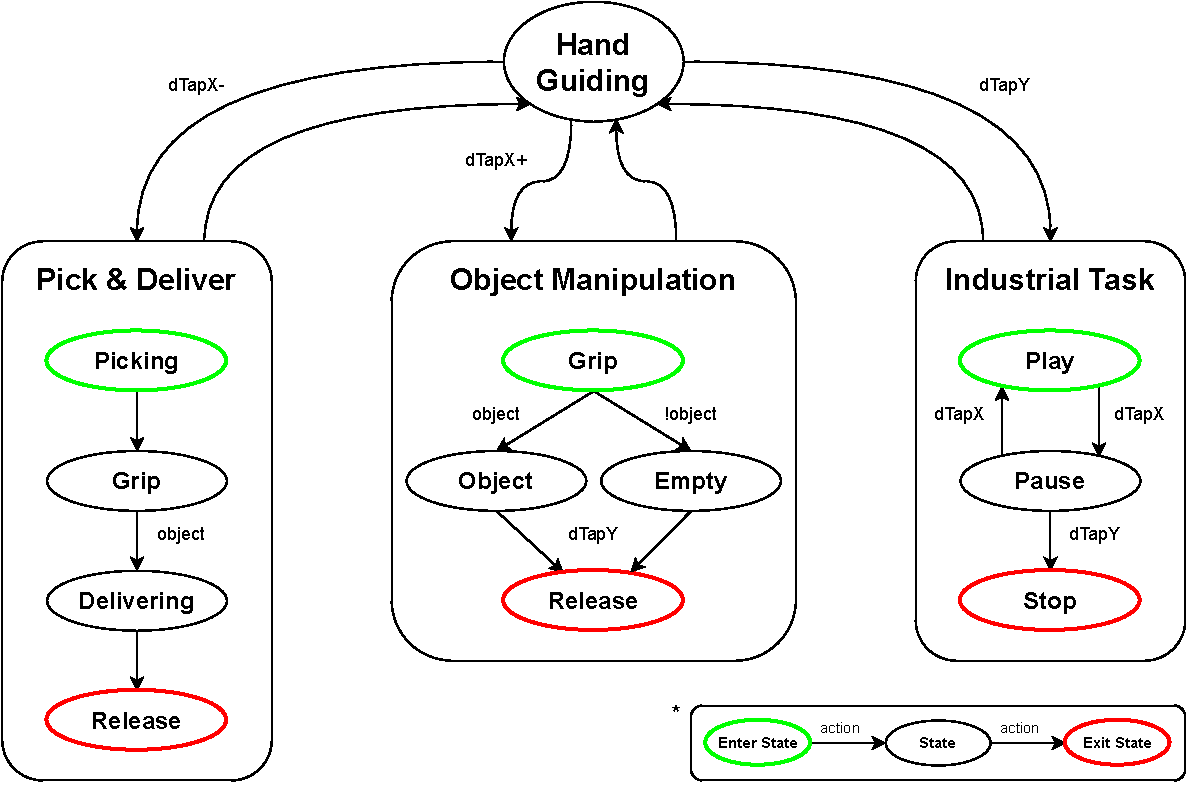
\includegraphics[width=0.8\linewidth]{figs/chp5/ros_ur10e_smach.pdf}
    \caption{\ac{ros} architecture of the compensation of \ac{ft} in real time}
    \label{fig:ros_smach}
\end{figure}

\begin{figure}[h]
    \centering
    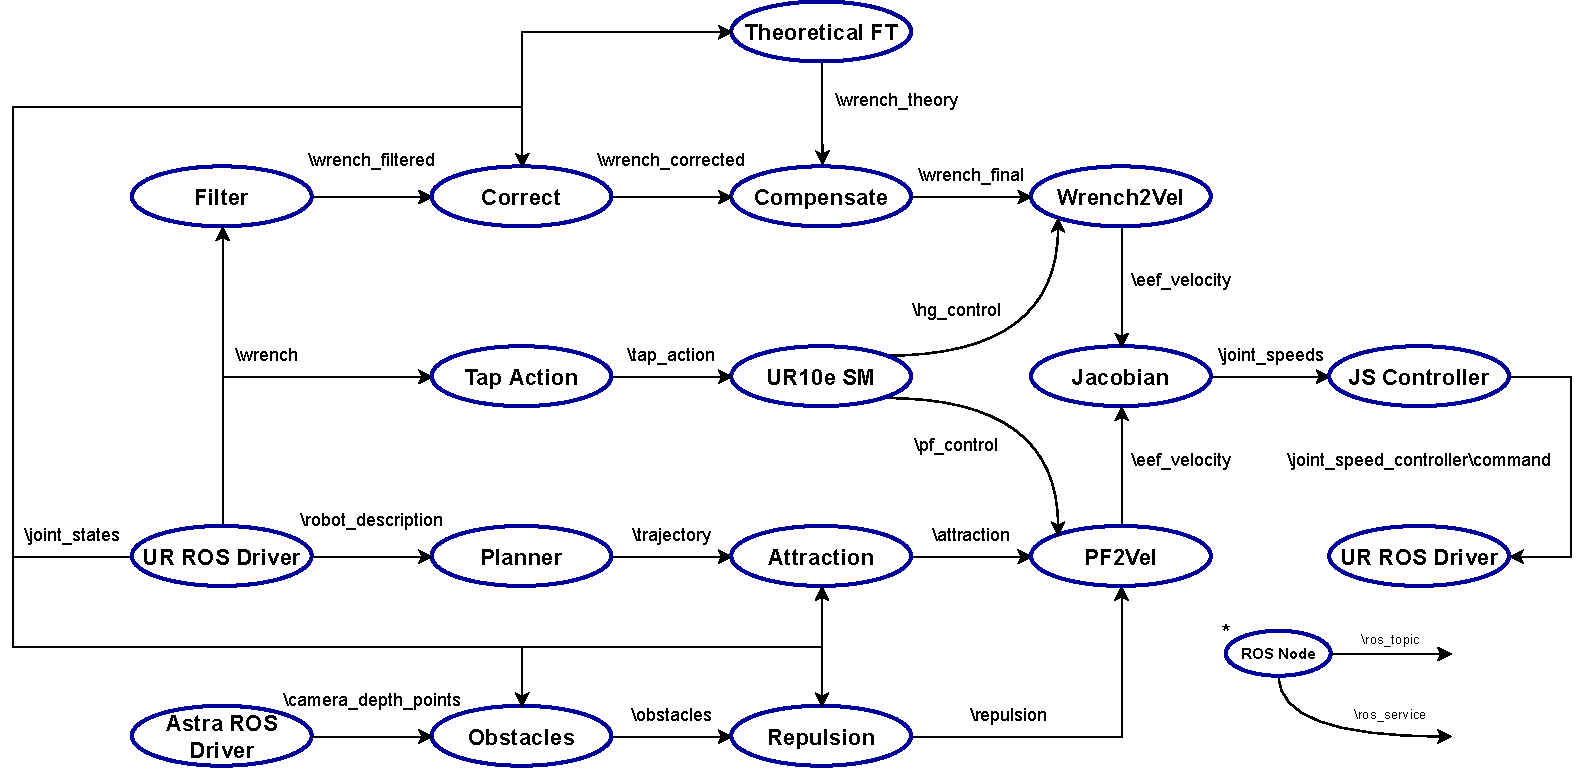
\includegraphics[width=\linewidth]{figs/chp5/ros_cobot_arch.pdf}
    \caption{\ac{ros} architecture of the compensation of \ac{ft} in real time}
    \label{fig:ros_cobot_arch}
\end{figure}


\subsection{State Transitions}

\par explain here the double tap interaction

\begin{figure}[h]
    \centering
    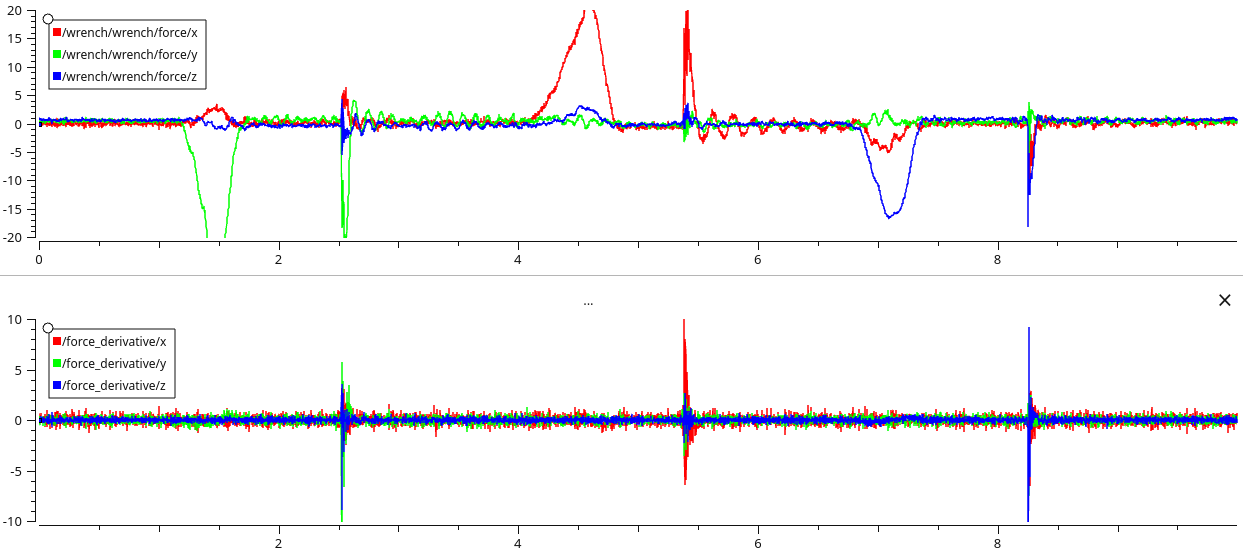
\includegraphics[width=0.9\linewidth]{figs/chp5/taps.png}
    \caption{Result of the compensation architecture applied in a real time test}
    \label{fig:taps}
\end{figure}

\subsection{Visual Feedback}

\par explain here the gripper color changing intergation

\begin{figure}[h]
    \centering
    \begin{subfigure}{.2\linewidth}
      \centering
      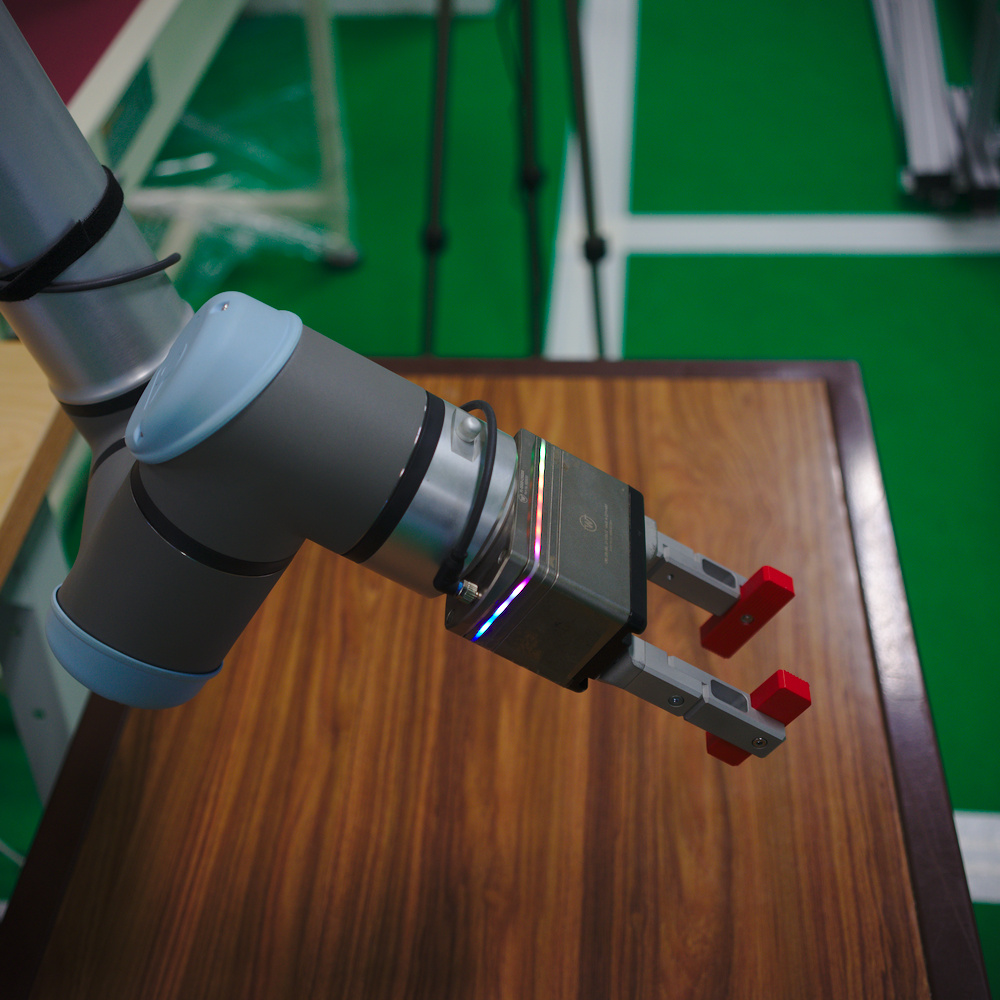
\includegraphics[width=.95\linewidth]{figs/chp5/grip_rgb.jpg}
    \end{subfigure}%
    \begin{subfigure}{.2\linewidth}
      \centering
      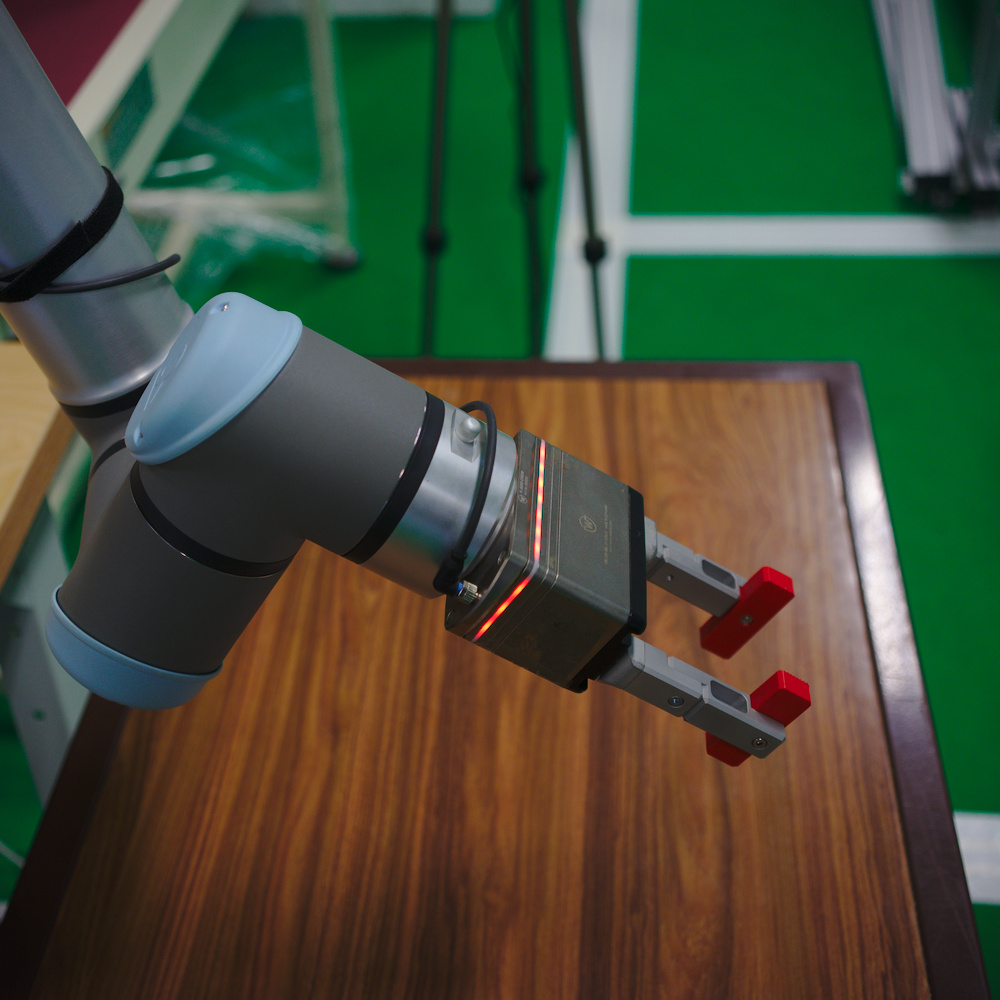
\includegraphics[width=.95\linewidth]{figs/chp5/grip_red.jpg}
    \end{subfigure}%
    \begin{subfigure}{.2\linewidth}
        \centering
        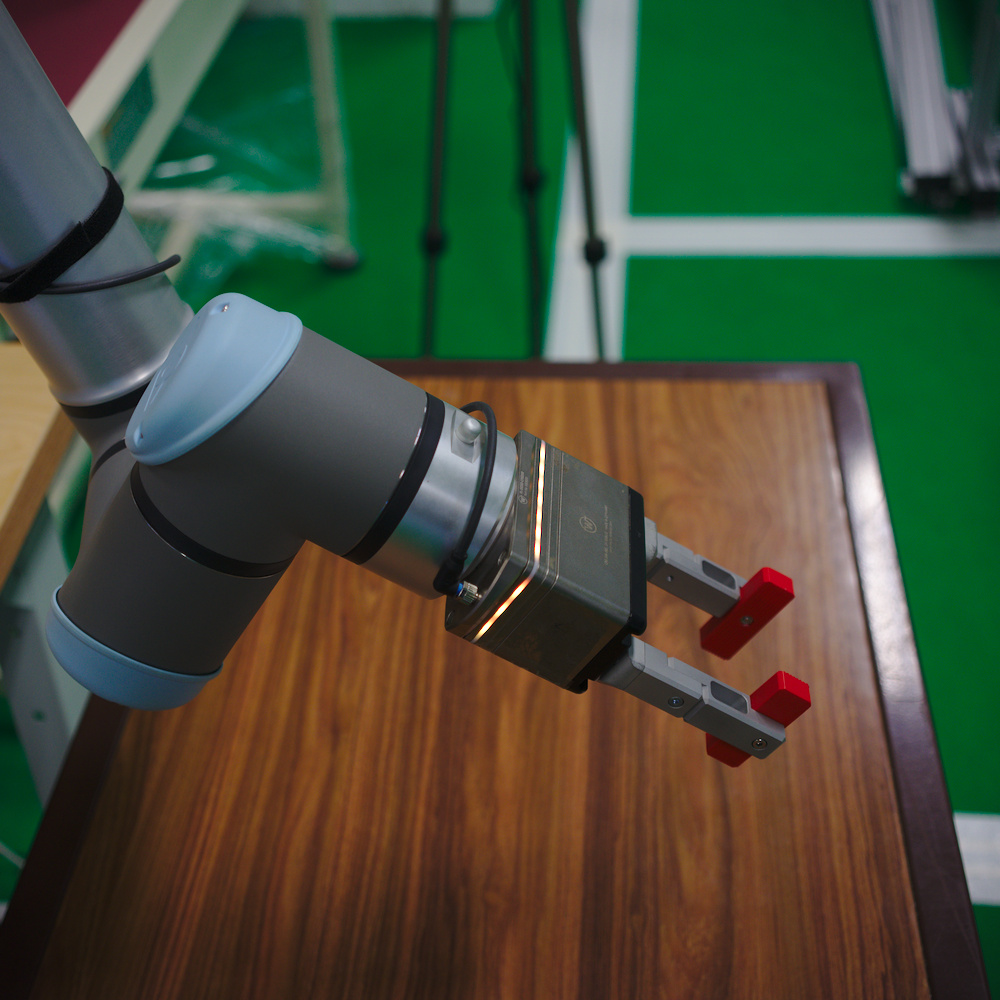
\includegraphics[width=.95\linewidth]{figs/chp5/grip_yellow.jpg}
    \end{subfigure}%
    \begin{subfigure}{.2\linewidth}
        \centering
        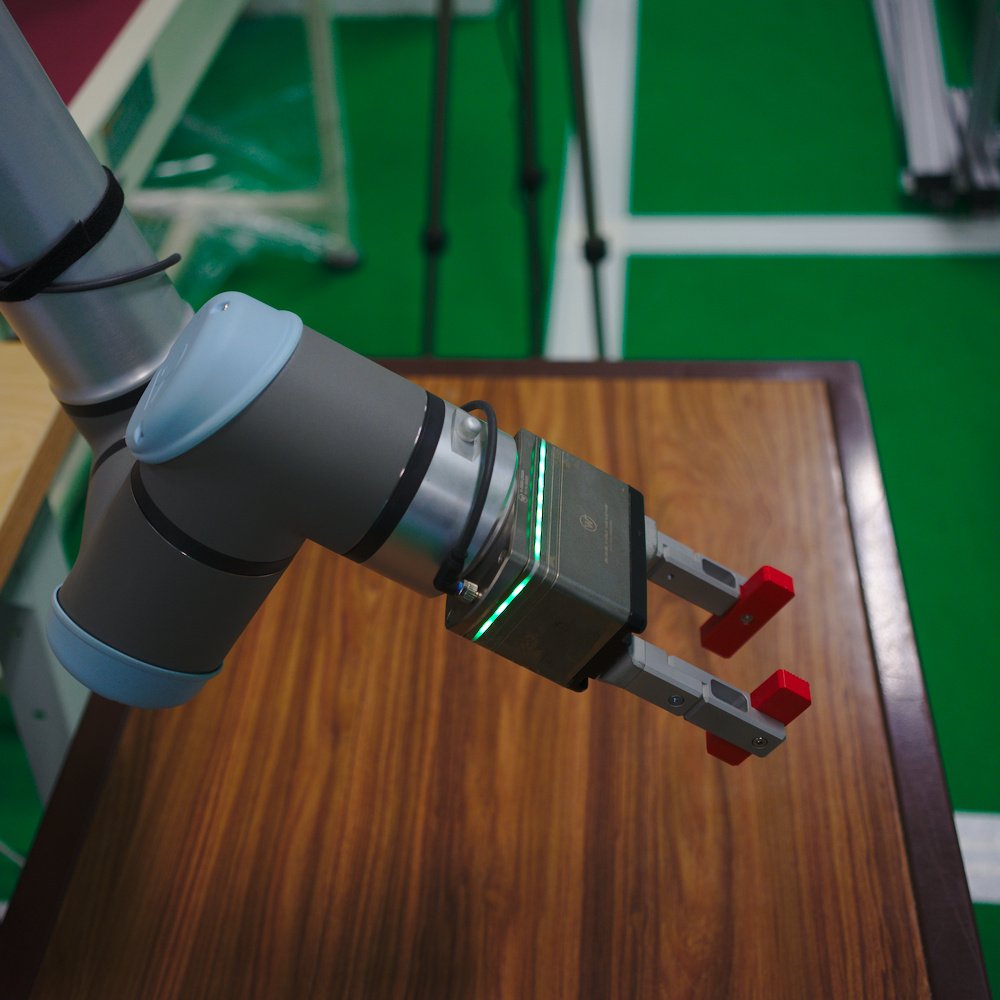
\includegraphics[width=.95\linewidth]{figs/chp5/grip_green.jpg}
    \end{subfigure}%
    \begin{subfigure}{.2\linewidth}
        \centering
        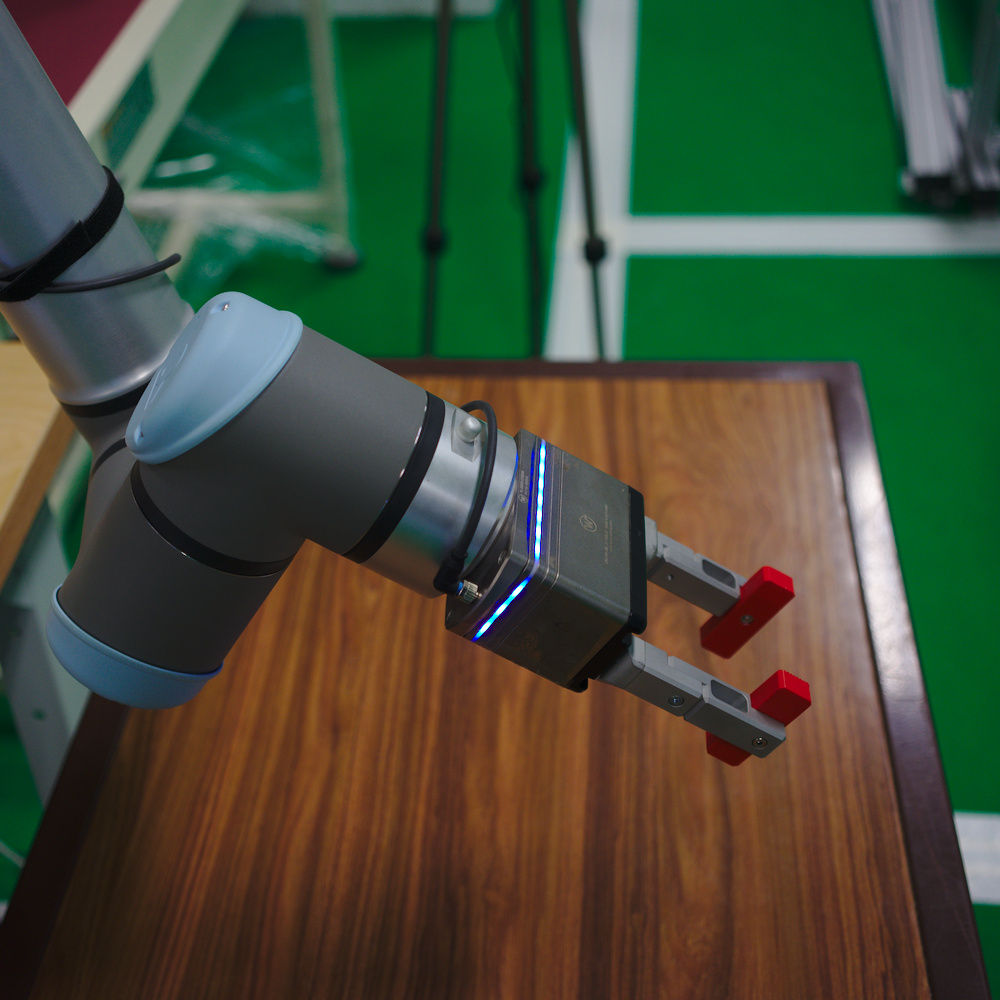
\includegraphics[width=.95\linewidth]{figs/chp5/grip_blue.jpg}
    \end{subfigure}
    \caption{\acs{led} status feedback on the gripper tool}
    \label{fig:gripper_leds}
\end{figure}


\section{Software Tools for \acs{hrc}}
\label{sec:tools-hrc}

\par iris\_sami
\par iris\_cobot
\par other viewers and tools such as plotjuggler integration and smach\_viewer
